% NIH Grant Proposal for the Specific Aims and Research Plan Sections
% LaTeX Template
% Version 1.1 (26/12/19)
%
% This template originates from:
% http://www.LaTeXTemplates.com
%
% Original author:
% Erick Tatro (erickttr@gmail.com) with modifications by:
% Vel (vel@latextemplates.com)
%
% Adapted from:
% J. Hrabe (http://www.magalien.com/public/nih_grants_in_latex.html)
%
% License:
% CC BY-NC-SA 3.0 (http://creativecommons.org/licenses/by-nc-sa/3.0/)
%
%%%%%%%%%%%%%%%%%%%%%%%%%%%%%%%%%%%%%%%%%

%----------------------------------------------------------------------------------------
%	PACKAGES AND OTHER DOCUMENT CONFIGURATIONS
%----------------------------------------------------------------------------------------

\documentclass[11pt, notitlepage]{article} % Default font size and suppress title page

\usepackage[utf8]{inputenc} % Required for inputting international characters
\usepackage[T1]{fontenc} % Output font encoding for international characters
% A note on fonts: As of 2019, NIH allows Arial, Georgia, Helvetica, and Palatino Linotype. Georgia and Arial are commercial fonts so you will need to use XeLaTeX and have them installed on your machine to use them. Palatino & Helvetica are available as free LaTeX packages so select the one you want and comment out the other.
\usepackage{palatino} % Palatino font
\linespread{1.05} % A little extra line spread is better for the Palatino font
%\usepackage{helvet} % Helvetica font
\renewcommand*\familydefault{\sfdefault} % Use the sans serif version of the font

\usepackage{amsfonts, amsmath, amsthm, amssymb} % For math fonts, symbols and environments
\usepackage{graphicx} % Required for including images
\usepackage{booktabs} % Nice rules in tables
\usepackage{wrapfig} % Required for text to wrap around figures and tables
\usepackage[labelfont=bf]{caption} % Make figure numbering in captions bold
\usepackage[top=0.5in,bottom=0.5in,left=0.5in,right=0.5in]{geometry} % Page margins

\usepackage{rotating}
\newcommand{\rulesep}{\unskip\ \vrule\ }

\usepackage[table,xcdraw]{xcolor}

% \pagestyle{empty} % Suppress headers and footers
\hyphenation{ionto-pho-re-tic iso-tro-pic fortran} % Specifies custom hyphenation points for words or words that shouldn't be hyphenated at all

%----------------------------------------------------------------------------------------

\begin{document}
\begin{center}
  \textbf{\Large{Proposta de Trabaho para Edital nº 09/2020}}
  \\
  \textbf{\Large{Prevenção e Combate a Surtos, Endemias, Epidemias e Pandemias}}
  \\
  \vspace{8pt}

  \textbf{Programa Pós Graduação em Informática}
  
  \vspace{8pt}
  \textbf{Aluno: Silas Pereira Lima Filho}

\textbf{Orientadoras: Jonice de Oliveira Sampaio, Mônica Ferreira da Silva}

\textbf{Linha de Pesquisa: Monitaramento da Saúde Mental em População Afetada pelo COVID-19}
\end{center}

%----------------------------------------------------------------------------------------
%	SPECIFIC AIMS
%----------------------------------------------------------------------------------------
\section*{Introdução}

A depressão é uma das doenças mentais mais relatadas no mundo. Algumas pessoas chamam de doença do século devido ao seu risco\footnote{www.theguardian.com/news/2018/jun/04/what-is-depression-and-why-is-it-rising}. 
A Organização \emph{Global Burden Disease} indica os transtornos depressivos como a terceira principal causa de incapacidade \cite{IHME}. Desde 1990, foi a quarta causa principal. 
Transtornos depressivos são indicados como a terceira principal causa de incapacidade\footnote{Disponível em http://ihmeuw.org/51aj}, como confirmado também por \cite{brody2018prevalence}. No entanto, em contraste com essa estabilidade, a depressão afeta certos grupos mais do que outros. Como mulheres para homens, europeus para africanos e pessoas com mais renda. É apresentado no Apêndice a Figura \ref{fig:depressionmap}, demonstrando essa estabilidade na evolução dos caos nos diferentes continentes.

A Organização Mundial de Saúde (OMS) apresenta que cerca de 300 milhões de pessoas de diferentes idades sofrem de algum nível de depressão\footnote{www.who.int/en/news-room/fact-sheets/detail/mental-disorders}. 
Alguns desses sintomas são, por exemplo, humor deprimido na maior parte do dia, perda de interesse em atividades regulares, perda de peso e insônia.
O Ministério da Saúde no Brasil apresenta que 11,5 milhões de pessoas são afetadas pela depressão\footnote{www.blog.saude.gov.br/index.php/materias-especiais/52516-mais-de-onze-milhoes-de-brasileiros-tem-depressao}.

É um desafio identificar pessoas doentes na fase inicial da depressão. Alguém depressivo pode enfrentar impedimentos como custo, preconceito social e até uma obstrução pessoal. Além disso, o caminho inverso também é um problema. Devido ao grande número de ocorrências de depressão, pode ser um obstáculo para institutos e profissionais alcançar aqueles que enfrentam uma doença mental e suas variantes. \cite{Lech2014} destaca a urgência na identificação e previsão precoces da depressão e seus sintomas devido às dificuldades em detectar esses sintomas nos estágios iniciais. \cite{elkin2008america} apresenta que 34\% da pesquisa em saúde é feita nas mídias sociais e 59\% dos adultos procuram informações sobre saúde na Internet.
Às vezes, devido à localização ou cenário econômico, o custo em obter ajuda de um profissional impossibilita alguém a procurar ajuda especializada.

O objetivo desse documento é apresentar informações e fatos que embasam a proposta de pesquisa que visa utilizar dados de mídias sociais para conseguir mensurar a saúde mental de pessoas usuárias de mídias sociais.

\subsection*{COVID-19 e suas Implicações}
O ano de 2020 é marcado pelo impacto do coronavírus na população mundial. O então definido pela comunidade científica, COVID-19, fez com que distintos grupos, economias e países adotassem o isolamento social como forma de controle da propagação da doença. Dado que sua tal doença é de alto contágio, atualmente, segundo o instituto John Hopkins, mais de 3 milhões pessoas foram contaminadas e mais de 100 mil pessoas faleceram devido à doença.\footnote{Dados conferidos em 13/08.}

Por conta da fácil propagação do COVID-19, os diferentes níveis de estado (Federal, Estado e Municipal) adotaram medidas para controle da doença. O que acarretou em uma adaptação da população criando então novos comportamentos. 
Comportamentos relacionados ao trabalho, formas de consumo, modos de relacionamento e outros tipos de atividades foram modificados por conta dos novos hábitos de comportamento delegados a população. Tais hábitos rodeiam o isolamento de pessoas e famílias. 

As variáveis que envolvem a pandemia ainda são analisadas tanto pela comunidade científica, mas também é debatida pelas pessoas fora dessa comunidade. Na população brasileira, existe a discussão popular sobre a eficácia das medidas adotadas e em muitos momentos as medidas tomadas pelas autoridades governamentais nem sempre se baseiam no conhecimento gerado pela comunidade científica.
Em meio a tantos fatores, de informação, conhecimento relacionados a doença, ainda é estudado que tipo de consequências cognitivas e psicológicas são geradas por conta da pandemia do COVID-19. Problemas como ansiedade, depressão vem a tona por conta tanto do medo de contaminação da doença que é facilmente propagável. Uma pessoa pode ter preocupações sobre o risco de contaminar-se, ou então ter preocupações sobre familiares ou pessoas próximas estarem em situação de delicada. O Instituto Brasileiro de Geografia e Estatística (IBGE) aponta que boa parte das empresas brasileiras tiveram um impacto negativo durante o período da pandemia\footnote{covid19.ibge.gov.br}. O que gera um impacto na empregabilidade e consequentemente criando uma preocupação em parte da população. 

\cite{PMID:32298802} realiza um  estudo utlizando questionários para medir o nível de estresse, ansiedade e depressão da população chinesa no período da pandemia. Os autores informam medidas que podem ser tomadas para minimizar o impacto na saúde mental, e também informa que dos grupos analisados, o que tem maior propensão a ter a saúde mental afetada é o de jovens e estudantes. \cite{wang2020immediate} também mede o impacto na saúde mental em relação ao nível de stress, ansiedade e depressão de grupos da população chinesa no período da pandemia. 

Em ambos os trabalhos citados, \cite{PMID:32298802} e \cite{wang2020immediate}, os autores sugerem que a identificação prévia dos grupos mais propensos a deselvoverem alguma doença psicológica, pode ajudar na adoção de medidas preventivas. 
Independemente da doença destacada nesse documento, o uso inteligente de informação e dados pode ajudar a identificar grupos de risco. Isso permite com que as devidas autoridades possam embasar sua tomada de decisões.

Alguns casos podem ser citados onde a tecnologia foi utilizada como forma de atenuar os problemas correlatos à pandemia. Em \cite{info:doi/10.2196/19292}, os autores medem a eficácia da utilização de mensagens SMS para dar apoio às pessoas e como forma de diminuir o stress. Já os autores de \cite{info:doi/10.2196/20185} medem as mudanças no comportamento de alunos universitários no período da pandemia. Os autores utilizam questionários para medir o nível de ansiedade e stress dos alunos, mas também medem o uso dos smartphone e.g. número de vezes em que o celular é destravado, distância percorrida etc. os autores analisam se tais medidas possuem correlação com as notícias sobre COVID-19.
Ye em \cite{info:doi/10.2196/19866} lista diversas formas de utilização da computação e informática no domínio da saúde. O autor sugere um framework chamado \emph{Tecnologia da Informação na Saúde} onde são mapeados as aplicações da computação. A Figura \ref{fig:HITframework} exibe tais divisões.

\begin{figure}[!ht]
  \centering
  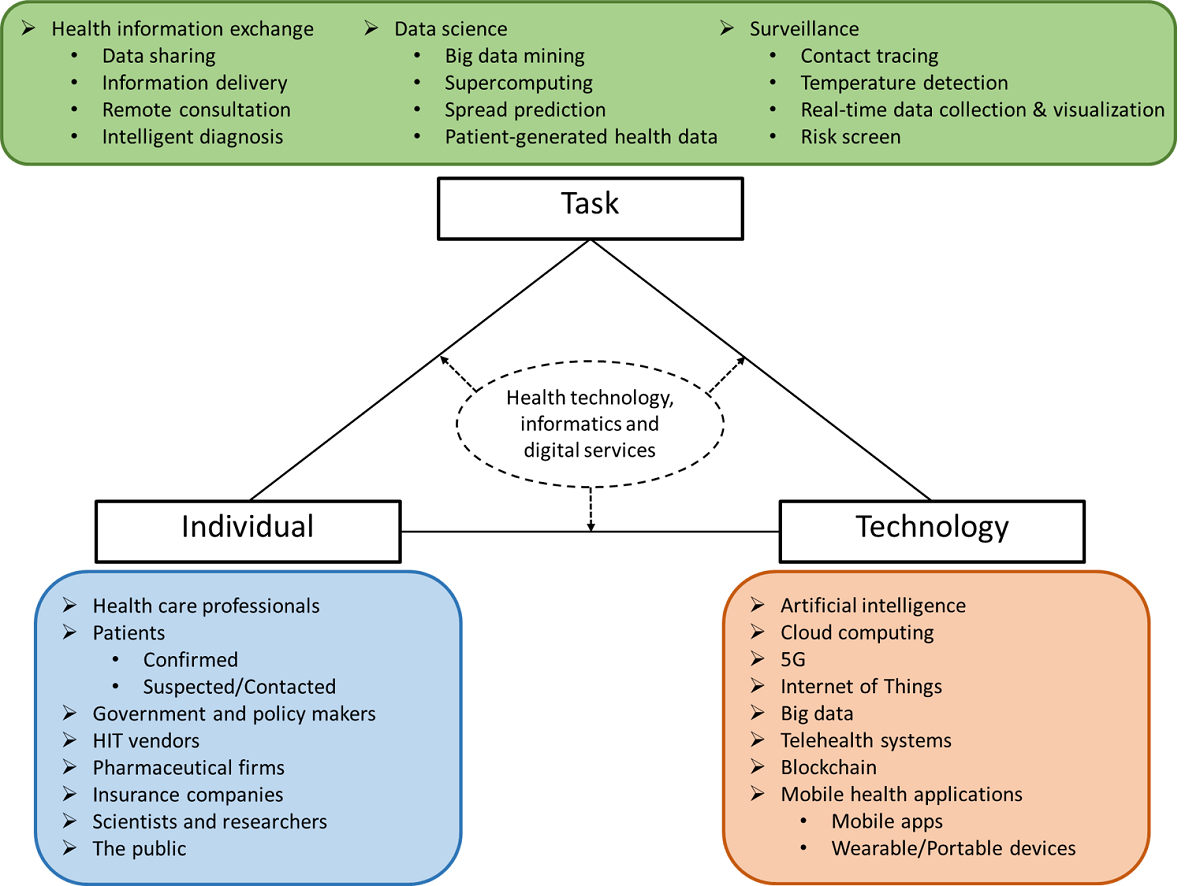
\includegraphics[scale=.45]{Figures/19866-391235-1-PB.png}
  \caption{Framework sugerido por \cite{info:doi/10.2196/19866}.}
  \label{fig:HITframework}
\end{figure}  

\subsection*{Monitoramento em Mídias Sociais}
\textit{Infodemiologia} e \textit{Detecção Digital de Doenças} são termos correlatos para descrever o uso de plataformas e ferramentas digitais para melhorar a saúde social. Eles podem ser traduzidos como esforços para combater epidemias, identificar indivíduos em risco e comunicar doenças urgentes de candidatos. O uso da tecnologia apóia diretamente instituições, profissionais e até ajuda as pessoas a se conscientizarem de algumas doenças \cite{Horvitz}.

Baseado em \cite{info:doi/10.2196/19866}, uma das tarefas listas é a análise de grandes conjuntos de dados. Com a coleta de informações sobre uma população e grupos, cria-se a chance de aproximar os recursos necessários para indivíduos em risco. Uma das tecnologias de coleta, e análise de grandes conjuntos de dados e que podem ser aplicados no domínio da saúde são as mídias sociais. Nelas, seus usuários publicam seus interesses e preferências sociais para então compartilhar com outros usuários. Elas se encaixam nos dois conceitos definidos acima. Podendo assim servir como fonte de informação e monitoramento para autoridades políticas e também para a comunidade científica. Podendo 
Através da mídia social, um usuário pode se conectar a seus amigos, parentes e até desconhecidos.
O conteúdo gerado nessas plataformas se parece com boas fontes de informação que podem ajudar ao lidar com a detecção ou conexão de doenças entre um psicólogo e um paciente depressivo.

\subsection*{Depressão}
% The 11th International Disease Classification (ICD 11) classifies depression as a disease when it is diagnosed in someone’s behavior. An event where the person has lost something e.g. job, some close person, etc. could start depression symptoms. This disease is also dangerous because of its extreme consequences. Depression, according to ICD 11, can lead to suicide ideation and suicide as consequence\cite{american2013diagnostic}. As a first step in order to investigate the problem of identification of depressive people on social media.

A 11ª Classificação Internacional de Doenças (CID 11) classifica a depressão como uma doença diagnosticada em relação ao comportamento de alguém. Um evento em que a pessoa perdeu algo, trabalho, alguma pessoa próxima, etc. podem iniciar sintomas de depressão. Esta doença também é perigosa por causa de suas consequências extremas. A depressão, segundo a CID 11, pode levar à ideação suicida e em consequência ao suicídio \cite{american2013diagnostic}.

Embora depressão seja o nome comum na sociedade, o Manual de Diagnóstico de Transtornos Mentais (DSM-V) detalha diferentes tipos de depressão. O mais comum e mais geral é o transtorno depressivo maior (TDM), embora cada variante da depressão seja coberta pelo termo \textit{Transtorno Depressivo}. As alternativas desse filho do transtorno são \textit{transtorno disruptivo da desregulação do humor}, \textit{Transtorno Depressivo Persistente (distimia)} e \textit{transtorno disfórico pré-menstrual}. O DSM-V também lista as características de diagnóstico de cada variante. Podemos listar critérios de diagnóstico de TDM, por exemplo insônia ou excesso de sono, humor depressivo na maior parte do dia, perda de interesse pelas atividades e perda de peso. O DSM-V também destaca que um grupo de pelo menos 5 sintomas deve ocorrer em um período de duas semanas.
Os sintomas e características da depressão são muito semelhantes à descrição de Freud da melancolia \cite{freud1917mourning}.

\subsection*{Dificuldades Tratamento da Depressão}
O diagnóstico da patologia se dá geralmente pela terapia, que é feita pela entrevista entre o profissional (psicólogo, psiquiatra ou médico). Atualmente, com a facilidade da tecnologia, profissionais da área da saúde adotaram ao \emph{teleatendimento} para conseguir atender pacientes remotamente. 
Cada região do cenário do serviço de saúde brasileiro possui suas particularidades. Num mesmo estado é possível encontrar grupos com grande poder aquisitivo, e outros que vivem em situação com recursos limitados.
Infelizmente, boa parte da população tem acesso limitado ao serviço de saúde. Muitas vezes por conta de desinformação ou por não conhecimento, não consegue tratamento médico profissional. Outras dificuldades para o tratamento de uma doença é a distância geográfica, ou então a disponibilidade de mão de obra em cidades nem sempre com muitos recursos, ou até mesmo preconceito de como pessoas próximas encaram uma possível doença psicológica. Todos esses fatores dificultam o trabalho de profissionais.

\subsection*{Detecção prévia de depressao}
Devido ao cenário descrito acima, identificar e atender alguém que possa ser um potencial paciente depressivo, de maneira rápida e discreta, parece ser muito útil tanto para o paciente quanto para o profissional. 
A tarefa de identificar alguma doença, mesmo que não seja depressão, pode ser desafiadora, mas ao mesmo tempo relevante. Investigar se é possível identificar sinais, sintomas de comportamento depressivo nas plataformas de mídia social. 
Devido à abundância de dados, pode tornar-se difícil o dado representativo. Portanto, escolha uma técnica confiável e uma análise consistente do método pode exigir uma grande quantidade de pesquisas.

% Como primeiro passo, a fim de investigar o problema de identificação de pessoas depressivas nas redes sociais.

% % 1 parágrafo - Depressão é considerada epidemia (o que é, crescimento a nível mundial, dados Brasil)
% % 1 parágrafo - Depressão x COVID 
% % isolamento e própria situação geral (desemprego, medo da morte, luto, isolamento, …) ajudado no aumento do número de casos. Referências!
% % Pandemia - dificuldade de tratamento 
% % 1 ou 2 parágrafos - Monitoração das mídias sociais tem ajudado na detecção de depressão - como? Colocar as referências
% % Detecção online da depressão, durante a pandemia, auxiliado a um teleatendimento pode salvar vidas
% \newpage

\section*{Proposta de Pesquisa}
% The proposed solution, in order to create an artifact, faces different stages that can offer challenges to the research to be accomplished. Since the final product is the hability to identify depression symptoms. We must pass by stages like obtain, process, model and persist the data from social network sites in a structure that can allow the further steps to retrieve this data for future analysis. Our method aims to identify a depressive user inserted in a social network in a reliable, consistent and unobtrusive manner. Figure \ref{fig:proposalgraph} depicts how we intend to achieve it. 

A solução proposta, para a criação de um artefato, enfrenta diferentes etapas que podem oferecer desafios à pesquisa a ser realizada. Já o produto final é a habilidade de identificar sintomas depressivos. Devemos passar por etapas como obter, processar, modelar e persistir os dados de sites de redes sociais em uma estrutura que possa permitir as próximas etapas para recuperar esses dados para análises futuras.
Nosso método visa identificar um usuário depressivo inserido em uma rede social de forma confiável, consistente e discreta. A Figura \ref{fig:proposalgraph} mostra um esquema conceitual de pretendemos organizar as etapas da pesquisa. 

\begin{figure}[!ht]
  \centering
  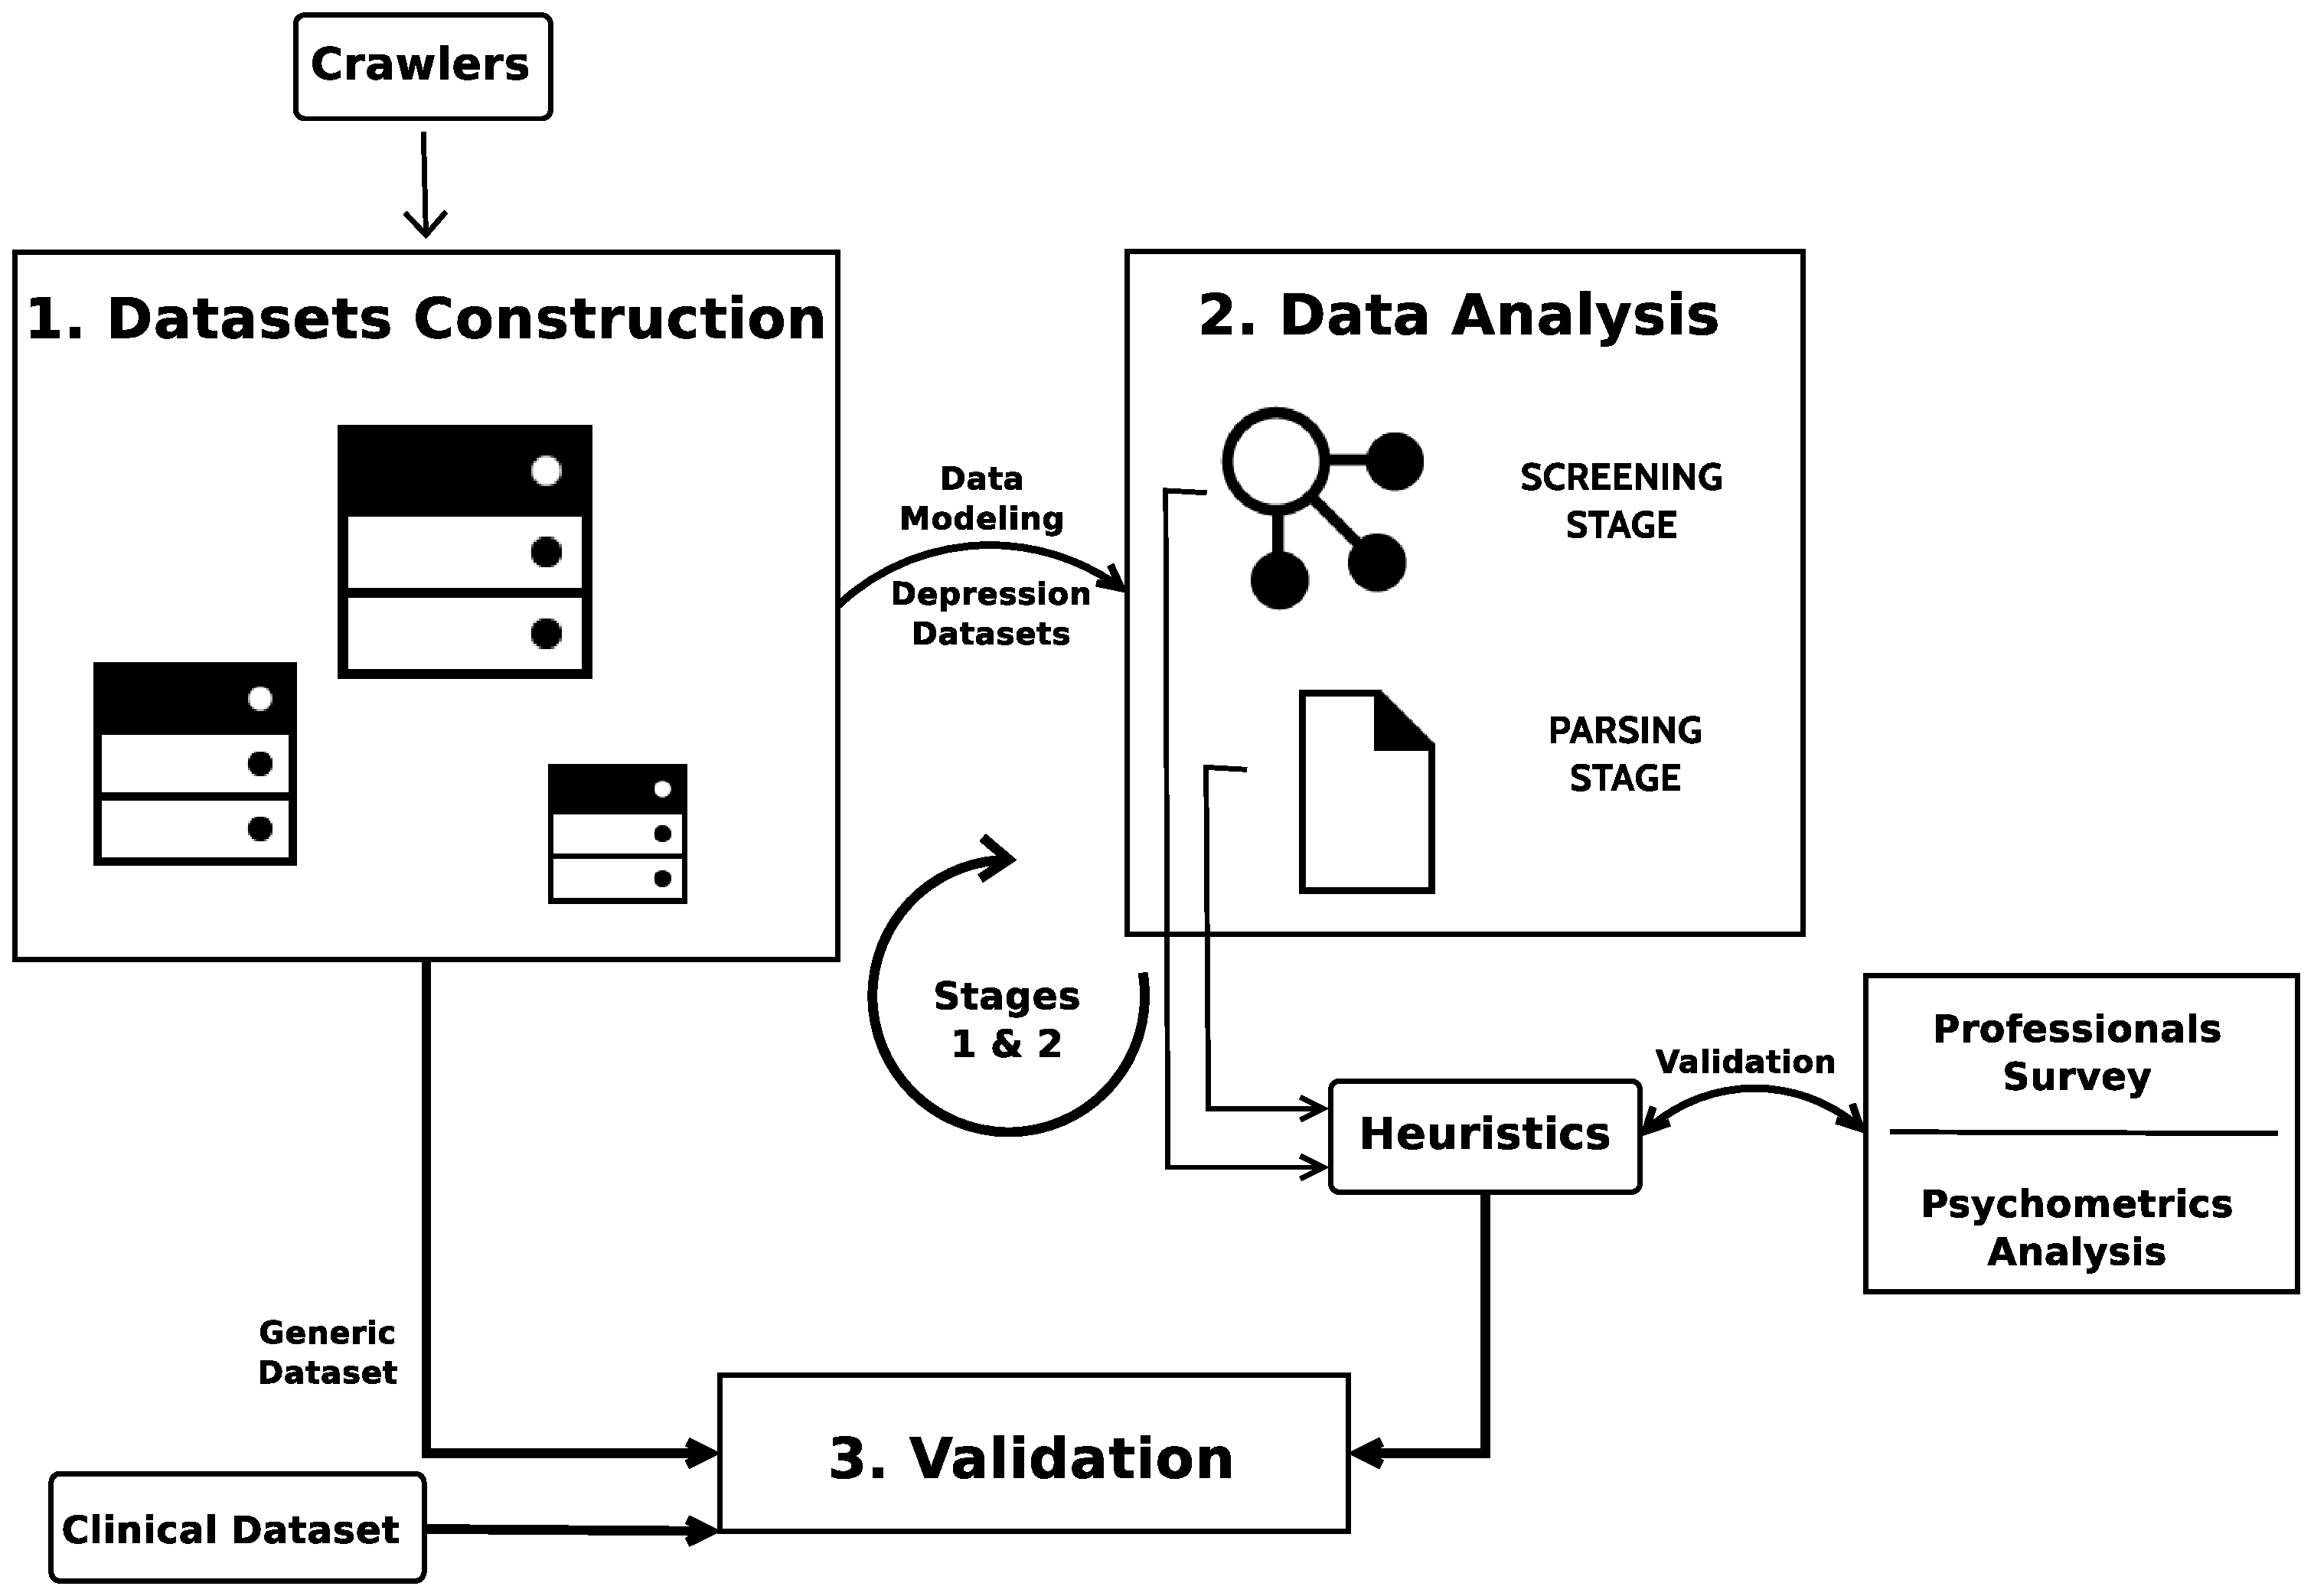
\includegraphics[keepaspectratio, width=.625\columnwidth]{Figures/conceptualModel.eps}
  \caption{Esquema conceitual da abordagem proposta.}
  \label{fig:proposalgraph}
\end{figure}

% Module 1 represents the phase where we construct the datasets to be explored in initial and later stages. This module is constructed mainly by crawlers and provides us depressive user's information concerning their vocabulary, content behavior and their preferences about relationships with other users. Afterwards datasets construction, through data modeling, Model 1 provides to Module 2 datasets from websites where depression is a key topic. The second module comprehends the data analysis and it splits this process into two substages. Both substages intend to abstract the implicit and explicit user's content. We represent Modules 1 and 2 as a cyclic process mainly due to the improvement of analysis, and evolution of datasets concerning length, complexity, and more abundat information.
O Módulo 1 representa a fase em que construímos os conjuntos de dados a serem explorados nos estágios iniciais e posteriores. Este módulo abrange a construção de datasets a serem analisados. Sua construção se dá por meio de crawlers e nos fornece informações sobre o usuário depressivo como seu vocabulário, comportamento de conteúdo e suas preferências sobre relacionamentos com outros usuários. Tais datasets devem possuir distintas proveniências para assim evitar um viés do dataset e consequentemente nas análises realizadas.
Atualmente, dois coletores foram desenvolvidos para obter dados dos sites \textit{HealingWell} e \textit{Reddit}. Por se tratar de uma pesquisa acadêmica, não temos a intenção de publicar os nomes dos autores e suas informações pessoais. No momento, temos um conjunto de dados com cerca de 1,5 GB de informações coletadas. O primeiro conjunto de dados está relacionado ao fórum de depressão do site da HealingWell \footnote{www.healingwell.com/community/default.aspx?f=19}. Coletamos 3075 tópicos postados e suas respectivas postagens, totalizando 18.450 postagens respondidas.

Posteriormente, a construção dos conjuntos de dados, por meio da modelagem de dados, o Modelo 1 fornece ao Módulo 2 conjuntos de dados de sites onde a depressão é um tópico chave. O segundo módulo compreende a análise dos dados e divide este processo em dois subestágios. Ambos os subestágios pretendem abstrair o conteúdo implícito e explícito do usuário. Os Módulos 1 e 2 são representados como um processo cíclico principalmente devido ao aprimoramento da análise e evolução dos conjuntos de dados em relação ao comprimento, complexidade e informações mais abundantes.  

% The screening substage comprehends a set of metrics that rely on topological analysis. Through social network analysis, we can understand how entities from a social network are connected. The topology study, through the use of social network analysis, can lead to the choice of specific users to have a better comprehension of them and their influence \cite{Razis2020}. We can list as examples three different types of relevant analysis, \textit{Social Influence Analysis}, \textit{Node Classification} and \textit{Community Detection} \cite{aggarwal2011socialnetwork}. With these analysis, it would be possible to have a better understanding of the connections around a depressive person.
O primeiro subestágio, de triagem, compreende um conjunto de métricas baseadas na análise topológica dos dados. Por meio da análise de redes sociais, podemos entender como as entidades de uma rede social estão conectadas. O estudo da topologia, através do uso da análise de redes sociais, pode levar à escolha de usuários específicos para melhor compreensão deles e sua influência \cite{Razis2020}. Podemos listar como exemplos três tipos diferentes de análises relevantes, \textit{Análise de Influência Social}, \textit{Classificação de Nó} e \textit{Detecção de Comunidade} \cite{aggarwal2011socialnetwork}. Com essas análises, seria possível ter um melhor entendimento das conexões em torno de uma pessoa depressiva. O trabalho de Rosenquist et.al. por exemplo consegue mapear dados de questionários psicométricos como grafos (que é a forma de representação de redes sociais). A partir de então os autores conseguem identificar o espalhamento da doença num determinado grupo \cite{Rosenquist2011}.

O subestágio de análise é dividido em três subprocessos e é representado na Figura \ref{fig:parsing_stage}. O processamento de linguagem natural (NLP) tem mostrado grande avanço nos últimos anos na análise de dados textuais. Modelos de linguagem tem sido utilizados para tarefas como a geração de conhecimento de um determinado domínio, extração de conhecimento em grandes conjuntos de texto, dentre outros. Uma das tarefas de NLP 
é a identificação automática dos tópicos de um texto. 
No subestágio de análise, aplicamos então as técnicas de análise textual nos dados coletados, o que se assemelha com outras abordagens científicas. Com base no trabalho de \cite{Nolasco2016}, pretendemos identificar quais são os principais tópicos de cada usuário em uma plataforma de mídia social. 
Após a identificação do tópico, para cada usuário, encontraremos a correlação entre os tópicos e mapearemos os termos em um gráfico de polaridade. 
O gráfico de polaridade pode ajudar a identificar se as palavras e os termos mais usados por um usuário tendem a ser positivos ou negativos.
Trabalhos relacionados mostraram que pessoas depressivas costumam manipular palavras mais negativas. Isso reflete a baixa autoestima desse grupo. Com os gráficos de polaridade de cada usuário, a terceira etapa pretende analisar como esses gráficos evoluíram. Dessa forma, será possível verificar se o discurso de alguém se tornou mais positivo ou negativo. A análise de séries temporais parece ser importante, visto que alguém é considerado deprimido se um conjunto de sintomas já ocorreu por um determinado período de tempo. Isso poderia ajudar a explicar melhor o fenômeno da depressão nas redes sociais.

\begin{figure}
  \centering
      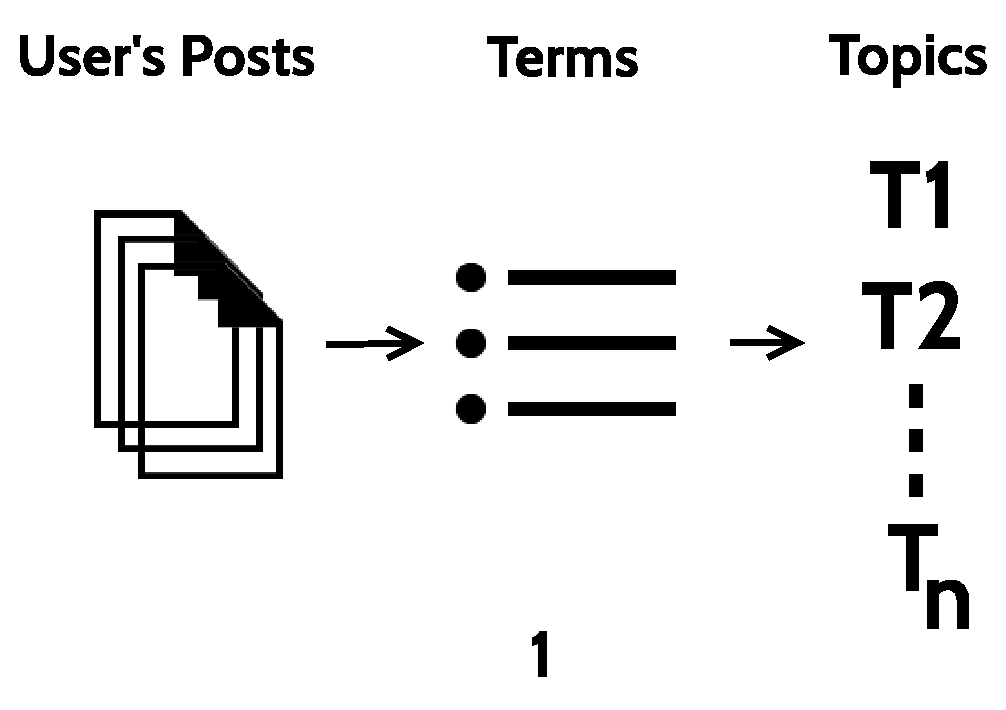
\includegraphics[trim=0 31 0 0, clip, width=0.265\textwidth]{Figures/method_1.eps} \hfill
      \rulesep
  % \centering
      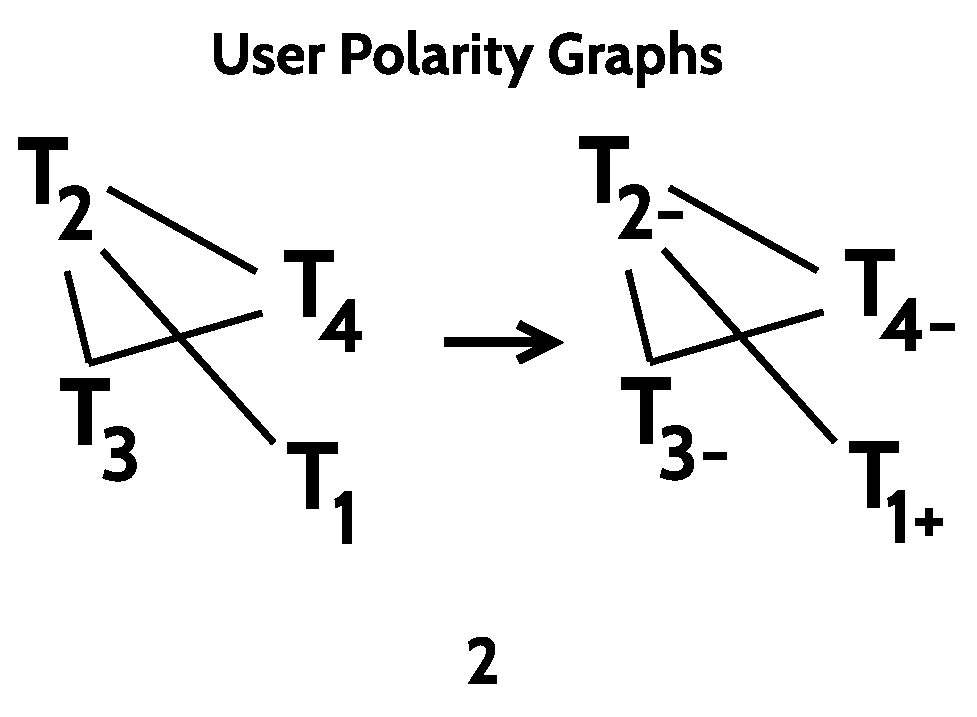
\includegraphics[trim=0 31 0 0, clip, width=0.265\textwidth]{Figures/method_2.eps} \hfill
      \rulesep
  % \centering
      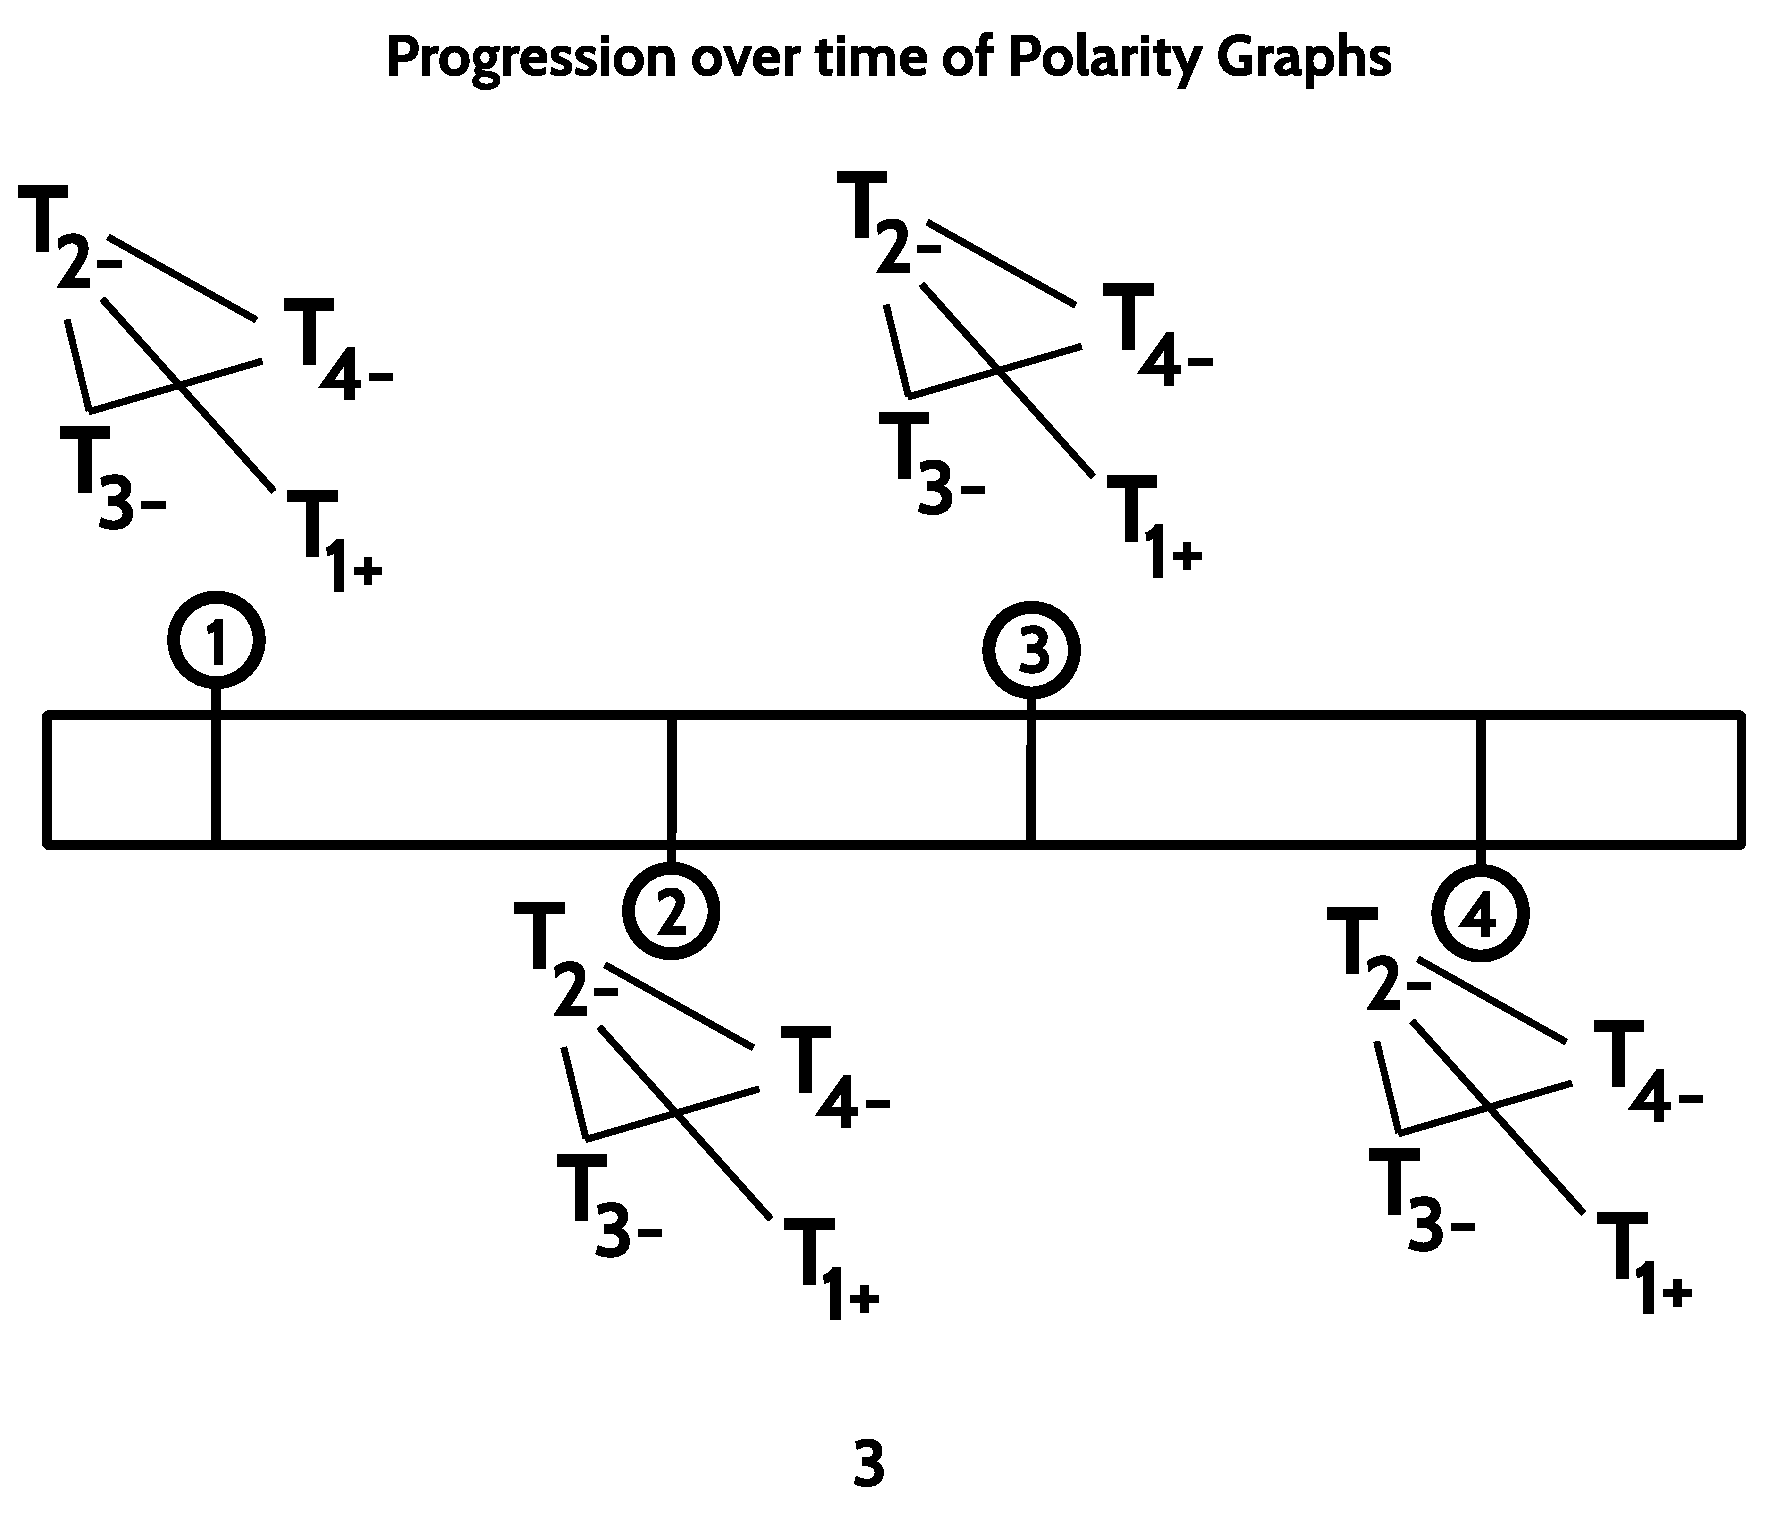
\includegraphics[trim=0 31 0 65, clip, width=0.265\textwidth]{Figures/method_3.eps} 

      % \caption{The Parsing stage's phases. Respectively, extraction of main topics from user content; Polarity of discovered topics; Evolution of polarity graphs over time.}
      \caption{As fases da etapa de Análise. Respectivamente, extração dos tópicos do conteúdo de um usuário; Polaridade dos tópicos descobertos; Evolução dos grafos de polaridade ao longo do tempo.}
      \label{fig:parsing_stage}
\end{figure}

À medida que as iterações progridem, o Módulo 2 constrói um conjunto de heurísticas extraídas da análise. Essas heurísticas são testadas por profissionais de pesquisa e comparadas à psicometria.
O conjunto de heurísticas também é validado no Módulo 3. Neste módulo, pretendemos validar as heurísticas não apenas aplicando-as em um conjunto de dados mais genérico e mais amplo, mas também testando em um cenário clínico de psicologia. Dessa forma, pretendemos corroborar a dinâmica e o comportamento da primeira iteração que foi abstraída de conjuntos de dados particulares.
% % (2 páginas) Proposta de Tese

\section*{Contribuições Esperadas}
A contribuição final esperada aumentar a área de conhecimento da computação na saúde mental. Devido às amplas implicações da depressão na saúde das pessoas e ao grande uso das mídias sociais, visa-se utilizar os dados coletados com maior precisão e confiabilidade para assim conseguir auxiliar profissionais e autoridades na tomada de decisões.
É proposto uma abordagem que difere sobre como lidar com a depressão com a ajuda de SNA e análise de texto.
Ressaltamos que a análise de redes sociais compreende a estrutura topológica. Portanto, a principal diferença em relação às pesquisas anteriores e à nossa proposta, é usar o conhecimento e as idéias da psicologia para melhorar o desempenho da classificação com SNA e análise textual.

Com esse experimento, iríamos entender o ambiente onde a doença depressão é o principal tópico de discussão, consequentemente, reproduziríamos e validaríamos os resultados e comportamentos das conversas sobre a depressão. A validação é principalmente dirigida à análise textual e de vocabulário. Embora pretendamos explorar profundamente a análise de redes sociais.

As etapas da metodologia proposta  As contribuições esperadas estão relacionadas à informática e à psicologia. Para a ciência da computação, esperamos que o emprego de métricas computacionais como análise de redes sociais e classificação de tópicos possa ajudar as pessoas a adquirir uma compreensão mais precisa de como o fenômeno da depressão acontece nas redes sociais e também como as redes sociais refletem a vida real.
Do ponto de vista da pesquisa em saúde (psicologia, medicina), nossa abordagem poderia melhorar a forma como o diagnóstico de depressão é realizado. Podendo assim ajudar as pessoas a terem uma saúde melhor por meio do uso da tecnologia.

\section*{Trabalhos Correlatos}
% For the literature selection, we have applied a systematic literature review \textbf{(SLR)} in order to have a deeper insight from the most recent research that tackles depression detection in social media. SLR allows to create protocols that can be reused by other researchers and therefore give to research transparency and reproducibility.
% It allows, whether the protocols are respected, 
% This stage is under construction yet and it is intended to include two more bases. The SLR until this moment was done searching for articles in ACM and IEEE bases. It has been searched the string \textit{(``Social Media" OR ``Social Network" OR ``Complex Network" ) AND (Depression OR ``Major Depressive Disorder")}. Including only works from 2013 until 2018, from computing area which have used social media as a data source. The inclusion and exclusion criteria are listed below in Table \ref{tab:rslCriterias}. At the final stage, there was a total number of 47 selected papers. There were 22 papers from ACM Library and 25 papers from IEEE Explore.

% \begin{center}
%   \begin{table}[h!]
%   \centering
%   \resizebox{.6\columnwidth}{!}{
%     \begin{tabular}{c|c}
%       \textbf{Inclusion}          & \textbf{Exclusion}                      \\ \hline
%       Directly tackles depression & Out of 2013-2018 scope                  \\ %\hline
%       Have computational approach & Not written in english or portuguese    \\ %\hline
%       Attend both approaches      & It is not a primary study               \\ %\hline
%       -                           & It does not have abstract               \\ %\hline
%       -                           & It does not have computing contribution \\ %\hline
%       -                           & It has less than 4 pages                \\ %\hline
%     \end{tabular}}
%     \caption{SLR Criterias for inclusion and exclusion.}
%     \label{tab:rslCriterias}
%   \end{table}
% \end{center}

% It may not seem clearly, but can be listed main objectives from read articles are: identify what symptoms are searchable in social media and will compose a model as features; create a model which classifies an unseen user as potential depressive or not. The problem of dealing with depression and social media can be understand as a search for people who suffer the symptoms of depression.
Pode não parecer claro, mas podem ser elencados os principais objetivos dos artigos lidos são: identificar quais sintomas são pesquisáveis nas mídias sociais e irão compor um modelo como recursos; criar um modelo que classifique um usuário invisível como potencial depressivo ou não. O problema de lidar com a depressão e as redes sociais pode ser entendido como uma busca por pessoas que sofrem os sintomas da depressão.

% A good amount of articles relies on natural language processing (NLP) to make a systemic analysis over the text in social media publications. Not all the analyzed researches take into account the psychology point of view. The effect of taking into account existing approaches from psychology is that the analysis will be more robust and reliable since the psychology research area already addresses mental disease problems. It is a challenge align quantification made by metrics e.g. NLP, social network analysis and other techniques to the cognition of a psychologist on ordinary clinical treatment. 
Uma boa quantidade de artigos se baseia em técnicas de NLP para fazer uma análise sistêmica do texto em publicações de mídia social. Nem todas as pesquisas analisadas levam em consideração o ponto de vista da psicologia. O efeito de levar em consideração as abordagens existentes da psicologia é que a análise será mais robusta e confiável, uma vez que a área de pesquisa da psicologia já aborda problemas de doenças mentais. É um desafio alinhar a quantificação feita por métricas. NLP, análise de redes sociais e outras técnicas para a cognição de um psicólogo em tratamento clínico comum.

% \cite{DeChoudhury:2013:SMM:2464464.2464480} has developed many articles and researches about the measurement of depression in population using social media information. The authors in this work have been made use of psychometrics questionnaires. Psychometrics represents the theory and technique of measuring mental processes and it is applied in Psychology and Education. It is an interesting approach, although it is questionable due to how it simplifies the whole process of understanding someone's behavior. In \cite{DeChoudhury:2013:SMM:2464464.2464480}, crowdsourcing is applied to obtain data from twitter by people who were clinically diagnosed with depression. With this data, they have constructed a corpus and developed a probabilistic model. The trained model classifies if a post indicates depression. Similar to previous work, Tsugawa et al \cite{Tsugawa2015} have applied the same analysis to replicate the results in a group of users from Japan.
\cite{DeChoudhury:2013:SMM:2464464.2464480} desenvolveu muitos artigos e pesquisas sobre a medição da depressão na população usando informações de mídia social. Os autores deste trabalho fizeram uso de questionários psicométricos.
A psicometria representa a teoria e a técnica de mensuração dos processos mentais e é aplicada na psicologia e na educação. É uma abordagem interessante, embora seja questionável por simplificar todo o processo de compreensão do comportamento de alguém. Em \cite{DeChoudhury:2013:SMM:2464464.2464480}, uma coleta no estilo crowdsourcing é aplicada para obter dados do Twitter por pessoas que foram clinicamente diagnosticadas com depressão. Com esses dados, eles construíram um corpus e desenvolveram um modelo probabilístico. O modelo treinado classifica se um post indica depressão. Semelhante ao trabalho anterior, Tsugawa et al \cite{Tsugawa2015} aplicaram a mesma análise para replicar os resultados em um grupo de usuários do Japão.

% \cite{Park:2015:MDL:2675133.2675139} present how activities on Facebook are associated with depressive states of users in order to raise awareness to depression at the University where the study was conducted, which had seen an increase in the suicide rate of its students. \cite{andalibi_sensitive_2017} explore self-disclosures posts in Instagram. In this article, the authors have used content from posts tagged with \#depression to understand what rather sensitive disclosures do people make on Instagram. The work in \cite{Li2016} is a qualitative study that tries to understand how is the behavior and comprehension of the Chinese population about depression. It is a qualitative study and differs from prior ones. \cite{Vedula2017} conduct an observational study to understand the interactions between clinically depressed users and their ego-network when contrasted with a group of users without depression. They identify relevant linguistic and emotional signals from social media exchanges to detect symptomatic cues of depression. \cite{Zhao:2018:TCM:3302425.3302501} have applied text classification using Convolutional Neural Networks to classify depression using text analysis. \cite{Nobles:2018:IIS:3173574.3173987} also have used neural networks to identify patterns on time periods when the risk of a suicide attempt is increasing in SMS texts. \cite{Yazdavar:2017:SAM:3110025.3123028} incorporate temporal analysis of user-generated content on social media for capturing symptoms. They have developed a statistical model that emulates traditional observational cohort studies conducted through online questionnaires and extract and categorize different symptoms of depression and modeling user-generated content in social media. \cite{Chen2018} detected eight basic emotions and calculated the overall intensity (strength score) of the emotions extracted from all past tweets of each user. After that, they have generated a time series for each emotion of every user in order to generate a selection of descriptive statistics for this time series.

\cite{Park:2015:MDL:2675133.2675139} apresenta como as atividades no Facebook estão associadas a estados depressivos de usuários a fim de aumentar a conscientização sobre a depressão na universidade onde o estudo foi realizado, que havia visto um aumento na taxa de suicídio de seus alunos. \cite{andalibi_sensitive_2017} explore postagens de auto-revelação no Instagram. Neste artigo, os autores usaram conteúdo de postagens marcadas com \emph{\#depression} para entender quais divulgações bastante confidenciais as pessoas fazem no Instagram. O trabalho in \cite{Li2016} é um estudo qualitativo que busca compreender como se dá o comportamento e a compreensão da população chinesa sobre a depressão. É um estudo qualitativo e difere dos anteriores. \cite{Vedula2017} conduz um estudo observacional para compreender as interações entre usuários clinicamente deprimidos e sua rede de ego quando comparados com um grupo de usuários sem depressão. Eles identificam sinais linguísticos e emocionais relevantes de intercâmbios de mídia social para detectar sinais sintomáticos de depressão. \cite{Zhao:2018:TCM:3302425.3302501} aplicou a classificação de texto usando Redes Neurais Convolucionais para classificar a depressão usando análise de texto. \cite{Nobles:2018:IIS:3173574.3173987} também usou redes neurais para identificar padrões em períodos de tempo em que o risco de tentativa de suicídio está aumentando em textos SMS. \cite{Yazdavar:2017:SAM:3110025.3123028} incorpora análise temporal de conteúdo gerado pelo usuário nas redes sociais para capturar sintomas. Eles desenvolveram um modelo estatístico que emula estudos de coorte observacionais tradicionais conduzidos por meio de questionários online e extraem e categorizam diferentes sintomas de depressão e modelam conteúdo gerado pelo usuário nas mídias sociais. \cite{Chen2018} detectou oito emoções básicas e calculou a intensidade geral (pontuação de força) das emoções extraídas de todos os tweets anteriores de cada usuário. Depois disso, eles geraram uma série temporal para cada emoção de cada usuário a fim de gerar uma seleção de estatísticas descritivas para esta série temporal.
% \silas{Paragraph below to highlight the aperture to investigate}

% Papers cited above not always take into account how psychologists infer if someone is depressive or not. We also stress that many of the real contributions rely on textual information generated by one user. Since one of the depression symptoms in ICD 11 is the inactivity, we could question if a depressive one would consistently generate online content. The context of psychology regularly deals with the subjectivity of information. Relied on that, we believe that relevant information can be extracted from other methods rather than text content. We believe that the classification of potential depressive users could be more reliable if combined with ``subjective information".
Os artigos citados acima nem sempre levam em consideração como os psicólogos inferem se alguém é depressivo ou não.
Ressaltamos também que muitas das contribuições reais dependem de informações textuais geradas por um usuário. Uma vez que um dos sintomas de depressão no CID 11 é a inatividade, poderíamos questionar se um sintoma depressivo geraria consistentemente conteúdo online. O contexto da psicologia lida regularmente com a subjetividade da informação. Com base nisso, acreditamos que informações relevantes podem ser extraídas de outros métodos, em vez de conteúdo de texto. Acreditamos que a classificação de potenciais usuários depressivos poderia ser mais confiável se combinada com ``informações subjetivas".

% (1 página) Trabalhos correlatos
% Mencionar brevmente os trabalhos correlatos e mencionar o seu diferencial
% Diferencial: Trabalhar com a identificação e monitoramento da VARIAÇÃO compartamental
\newpage
\section*{Cronograma}
O período estipulado para a proposta apresentada é de 36 meses. A Tabela \ref{tab:Cronograma} apresenta as etapas estipuladas para a pesquisa. Destaca-se que o cronograma apresentado poderá flexibilizar-se de modo a atender as demandas de tempo da chamada de trabalho. Basicamente é intencionado que a pesquisa se desenvolva no principalmente nos dois primeiros anos. Assim, nos últimos doze meses é esperado um trabalho mais focado na divulgação acadêmica e científica dos dados analisados e do conhecimento gerado por meio da pesquisa.


\begin{table}[!ht]
  \centering
  \begin{tabular}{cllll}
  \hline
% CABECALHO
  \multicolumn{5}{|c|}{\cellcolor[HTML]{C0C0C0}\textbf{\large{Primeiro Ano - De 09/2020 a 09/2021}}} \\ \hline
  \multicolumn{1}{|c|}{\cellcolor[HTML]{C0C0C0}\textbf{Atividades}} & \multicolumn{4}{c|}{\cellcolor[HTML]{C0C0C0}\textbf{Quartis}} \\ \hline
  \multicolumn{1}{|c|}{} & \multicolumn{1}{c|}{Q.1} & \multicolumn{1}{c|}{Q.2} & \multicolumn{1}{c|}{Q.3} & \multicolumn{1}{c|}{Q.4} \\ \hline

  \multicolumn{1}{|c|}{Revisão Bibliográfica} & \multicolumn{1}{c|}{X} & \multicolumn{1}{c|}{} & \multicolumn{1}{c|}{} & \multicolumn{1}{c|}{} \\ \hline
  \multicolumn{1}{|c|}{Criação de coletores de dados} & \multicolumn{1}{c|}{} & \multicolumn{1}{c|}{X} & \multicolumn{1}{c|}{} & \multicolumn{1}{c|}{} \\ \hline
  \multicolumn{1}{|c|}{Qualificação de Tese} & \multicolumn{1}{c|}{} & \multicolumn{1}{c|}{X} & \multicolumn{1}{c|}{} & \multicolumn{1}{c|}{} \\ \hline
  \multicolumn{1}{|c|}{Aplicação de Survey com profissionais da saúde} & \multicolumn{1}{c|}{} & \multicolumn{1}{c|}{} & \multicolumn{1}{c|}{X} & \multicolumn{1}{c|}{} \\ \hline
  \multicolumn{1}{|c|}{Análise Topológica dos Dados} & \multicolumn{1}{c|}{} & \multicolumn{1}{c|}{} & \multicolumn{1}{c|}{X} & \multicolumn{1}{c|}{} \\ \hline
    \multicolumn{1}{|c|}{Análise de Dados Textuais} & \multicolumn{1}{c|}{} & \multicolumn{1}{c|}{} & \multicolumn{1}{c|}{} & \multicolumn{1}{c|}{X} \\ \hline
  \multicolumn{1}{|c|}{Validação de Análises Realizadas} & \multicolumn{1}{c|}{} & \multicolumn{1}{c|}{} & \multicolumn{1}{c|}{} & \multicolumn{1}{c|}{X} \\ \hline
  
  
% CABECALHO
  \multicolumn{5}{|c|}{\cellcolor[HTML]{C0C0C0}\textbf{\large{Segundo Ano - De 10/2021 a 10/2022}}} \\ \hline
  \multicolumn{1}{|c|}{\cellcolor[HTML]{C0C0C0}\textbf{Atividades}} & \multicolumn{4}{c|}{\cellcolor[HTML]{C0C0C0}\textbf{Quartis}} \\ \hline
  \multicolumn{1}{|c|}{} & \multicolumn{1}{c|}{Q.1} & \multicolumn{1}{c|}{Q.2} & \multicolumn{1}{c|}{Q.3} & \multicolumn{1}{c|}{Q.4} \\ \hline

  \multicolumn{1}{|c|}{Atualização da Revisão Bibliográfica} & \multicolumn{1}{c|}{X} & \multicolumn{1}{c|}{} & \multicolumn{1}{c|}{} & \multicolumn{1}{c|}{} \\ \hline
  \multicolumn{1}{|c|}{Criação de modelo de classificação inicial} & \multicolumn{1}{c|}{X} & \multicolumn{1}{c|}{} & \multicolumn{1}{c|}{} & \multicolumn{1}{c|}{} \\ \hline
  \multicolumn{1}{|c|}{Validação de Performance do Modelo} & \multicolumn{1}{c|}{X} & \multicolumn{1}{c|}{} & \multicolumn{1}{c|}{} & \multicolumn{1}{c|}{} \\ \hline
  \multicolumn{1}{|c|}{Validação de Análises Realizadas} & \multicolumn{1}{c|}{} & \multicolumn{1}{c|}{X} & \multicolumn{1}{c|}{} & \multicolumn{1}{c|}{} \\ \hline
  
  
  \multicolumn{1}{|c|}{Aplicação de survey com pacientes depressivos} & \multicolumn{1}{c|}{} & \multicolumn{1}{c|}{X} & \multicolumn{1}{c|}{X} & \multicolumn{1}{c|}{} \\ \hline
  \multicolumn{1}{|c|}{Análise de dados do survey} & \multicolumn{1}{c|}{} & \multicolumn{1}{c|}{} & \multicolumn{1}{c|}{X} & \multicolumn{1}{c|}{X} \\ \hline
  
  \multicolumn{1}{|c|}{Validação de Heurísticas} & \multicolumn{1}{c|}{} & \multicolumn{1}{c|}{} & \multicolumn{1}{c|}{} & \multicolumn{1}{c|}{} \\ \hline
  \multicolumn{1}{|c|}{Escrita de Tese} & \multicolumn{1}{c|}{X} & \multicolumn{1}{c|}{X} & \multicolumn{1}{c|}{X} & \multicolumn{1}{c|}{X} \\ \hline
  \multicolumn{1}{|c|}{Defesa Tese} & \multicolumn{1}{c|}{} & \multicolumn{1}{c|}{} & \multicolumn{1}{c|}{} & \multicolumn{1}{c|}{X} \\ \hline
% CABECALHO
  \multicolumn{5}{|c|}{\cellcolor[HTML]{C0C0C0}\textbf{\large{Terceiro Ano - De 10/2022 a 09/2023}}} \\ \hline
  \multicolumn{1}{|c|}{\cellcolor[HTML]{C0C0C0}\textbf{Atividades}} & \multicolumn{4}{c|}{\cellcolor[HTML]{C0C0C0}\textbf{Quartis}} \\ \hline
  \multicolumn{1}{|c|}{} & \multicolumn{1}{c|}{Q.1} & \multicolumn{1}{c|}{Q.2} & \multicolumn{1}{c|}{Q.3} & \multicolumn{1}{c|}{Q.4} \\ \hline

  \multicolumn{1}{|c|}{Atualização da Revisão Bibliográfica} & \multicolumn{1}{c|}{X} & \multicolumn{1}{c|}{} & \multicolumn{1}{c|}{} & \multicolumn{1}{c|}{} \\ \hline
  \multicolumn{1}{|c|}{Submissão para Journal (A definir)} & \multicolumn{1}{c|}{X} & \multicolumn{1}{c|}{X} & \multicolumn{1}{c|}{X} & \multicolumn{1}{c|}{X} \\ \hline
  \multicolumn{1}{|c|}{Submissão para Congresso (A definir)} & \multicolumn{1}{c|}{X} & \multicolumn{1}{c|}{X} & \multicolumn{1}{c|}{X} & \multicolumn{1}{c|}{X} \\ \hline
  

  \end{tabular}
  \caption{Cronograma da proposta de pesquisa.}
  \label{tab:Cronograma}
  \end{table}

%----------------------------------------------------------------------------------------
%	BIBLIOGRAPHY
%----------------------------------------------------------------------------------------

\newpage
\bibliography{bibliografia} % Use the NIHGrant.bib file for the reference list, replace with your own
\bibliographystyle{nihunsrt} % Use the custom nihunsrt bibliography style included with the template

%----------------------------------------------------------------------------------------
\appendix
\begin{sidewaysfigure}
	\centering
	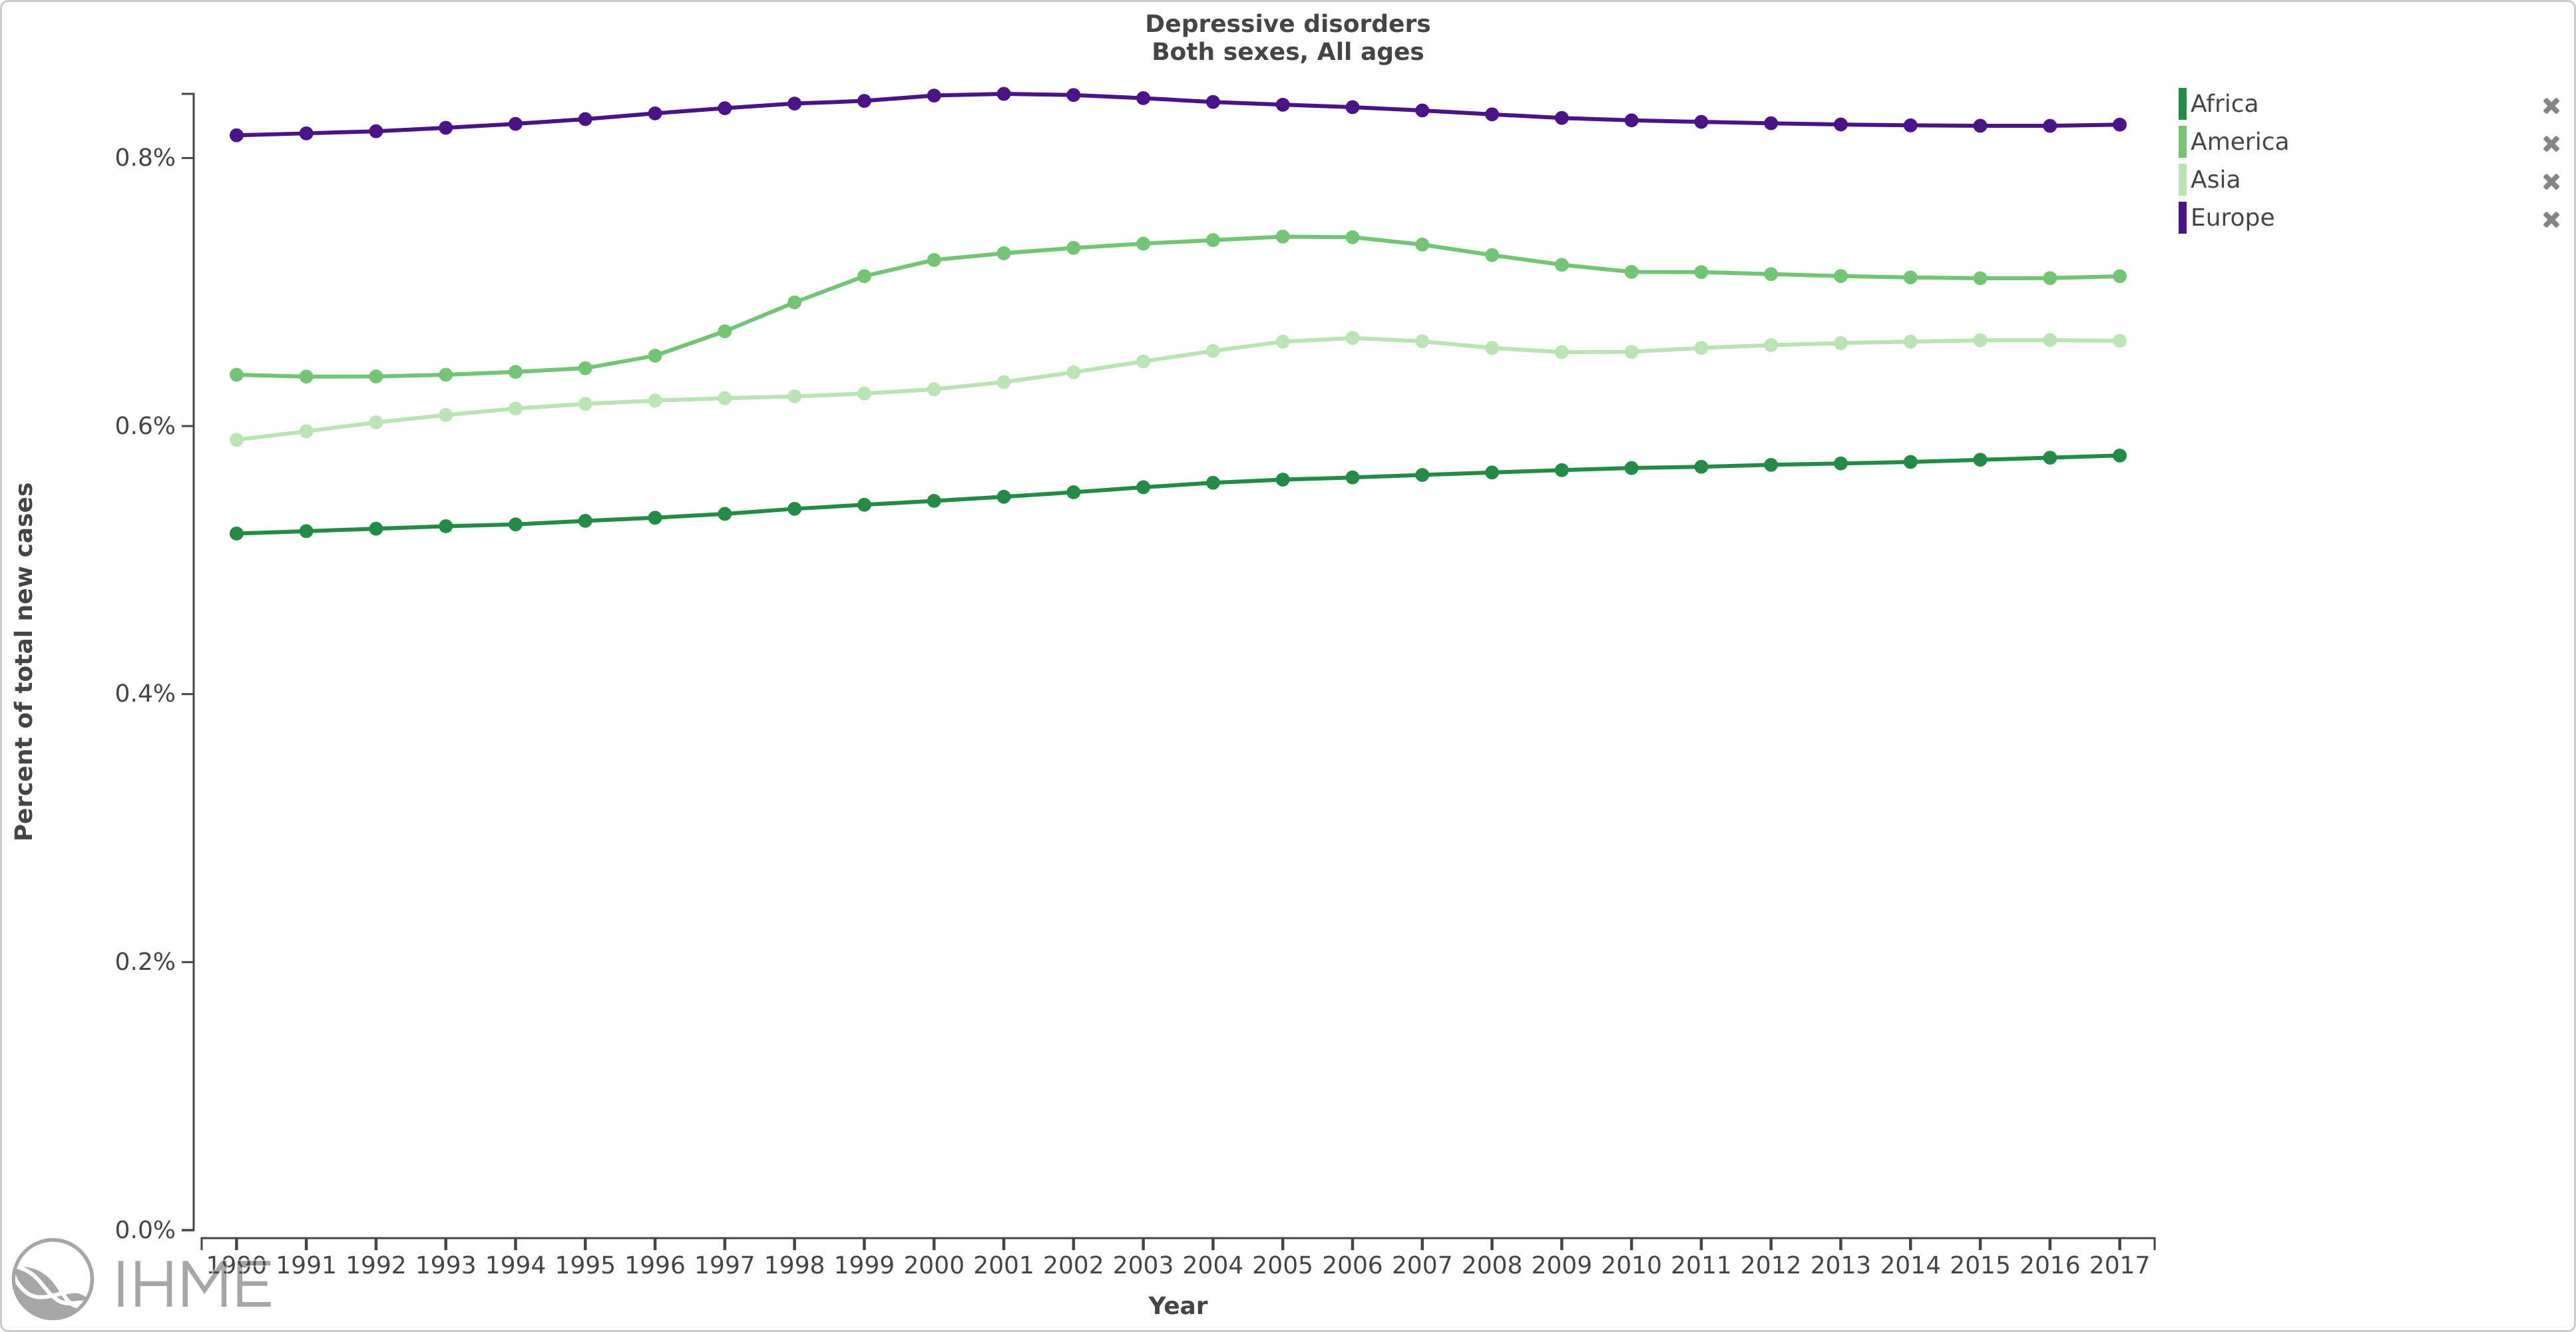
\includegraphics[scale=.24]{Figures/depressionprogression.png}
	\caption{Depression progression over the years by global regions} 
	\label{fig:depressionmap}
\end{sidewaysfigure}
%----------------------------------------------------------------------------------------
\end{document}

